\documentclass[10pt]{article}
\usepackage[a4paper,top=1pt,bottom=2pt,left=1pt,right=1pt,marginparwidth=1pt,headheight=1pt]{geometry}
% Encoding Settings
\usepackage[T1]{fontenc}
\usepackage[utf8]{inputenc}



% Font Settings
\usepackage{times}

% Define a new font called Tinyb. This font can maintain its shape even in very small fontsize:
% \usepackage{lmodern}
% \rmfamily
% \DeclareFontShape{T1}{lmr}{bx}{sc}{<-> cmr10}{}% USE BOLD SCSHAPE NOT OTHERWISE DEFINED
% %%% MATH FONT FIX
% \DeclareFontFamily{OML}{zlmm}{}
% \DeclareFontShape{OML}{zlmm}{m}{it}{<-> lmmi10}{}
% \DeclareFontShape{OML}{zlmm}{b}{it}{<->ssub * zlmm/m/it}{}
% \DeclareFontShape{OML}{zlmm}{bx}{it}{<->ssub * zlmm/m/it}{}
% \DeclareMathVersion{Tinyb}
% \SetSymbolFont{operators}{Tinyb}{T1}{lmr}{bx}{sc}
% \SetSymbolFont{letters}{Tinyb}{OML}{zlmm}{m}{it}
% \newenvironment{tinyb}{\bgroup\tiny\bfseries\scshape\mathversion{Tinyb}}{\egroup}



% Paragraph Settings
\usepackage{setspace}
\onehalfspacing
\usepackage{parskip}
\setlength{\parindent}{0in}



% Reference Settings
\usepackage[
    backend=biber,
    style=ieee,
]{biblatex}
\addbibresource{References.bib}

% Elegantly break long doi field
% \setcounter{biburllcpenalty}{100}
% \setcounter{biburlucpenalty}{100}
% \setcounter{biburlnumpenalty}{100}



% Figure Settings
\usepackage{graphicx} % Required for inserting images
\renewcommand{\figurename}{\textbf{Fig.}}

\usepackage{float}

% Enable two figures in one line:
% \usepackage{subfig}
% \begin{figure}[htbp!]
%   \centering
%   \subfloat[Before re-initialization]{\includegraphics[width=0.5\textwidth]{Figures/Before re-initialization.pdf}\label{fig:f1}}
%   \hfill
%   \subfloat[After re-initialization]{\includegraphics[width=0.5\textwidth]{Figures/After re-initialization.pdf}\label{fig:f2}}
%   \centering
%   \caption{Swarm distribution before and after reinitializing transitional particles on a one-dimensional problem}
%   \label{fig:before_and_after_reinitialization}
% \end{figure}



% Array Settings
\usepackage{array}
\newcolumntype{R}{>{$}r<{$}} % math-mode version of "r" column type
\newcolumntype{C}{>{$}c<{$}} % math-mode version of "c" column type
\newcolumntype{L}{>{$}l<{$}} % math-mode version of "l" column type

% defines a new type of column called Y based on a X column (this column type is defined by the tabularx package and it is basically a p{ <width>} column, where <width> is calculated by the package) but typesets the content using \small font size and with ragged-right text.
% \newcolumntype{Y}{>{\small\raggedright\arraybackslash}X}

% Modify the space on the bottom and top of each cell:
\usepackage{cellspace}
% \addtolength{\cellspacetoplimit}{5pt}
% \addtolength{\cellspacebottomlimit}{5pt}

\usepackage{multirow}
\usepackage{tabularx,booktabs}
\usepackage{longtable}
\usepackage{relsize}

% \renewcommand{\thetable}{S\arabic{table}}  % Rename the table names to Table Sx.

% Equally spread columns to fulfill the whole table.
% \begin{longtable}[c]{@{\extracolsep{\fill}}Lllllllll}

% Define a horizontal line that only appears in specific columns:
% \usepackage{hhline}
% \hhline{~----~~}  % Use as \hline, but the column with ~ will not have a horizontal line.



% Hyper-reference Settings
\usepackage{hyperref}
\hypersetup{
    colorlinks=true,
    linkcolor=cyan,
    citecolor=cyan,
    urlcolor=cyan,
}
% \usepackage[all]{hypcap} 
% \makeatletter
% \AtBeginDocument{\def\@citecolor{cyan}}  % Define citing 
% \AtBeginDocument{\def\@urlcolor{cyan}}
% \AtBeginDocument{\def\@linkcolor{cyan}}
% \makeatother

% Make the brackets of equation citation blue:
% \hyperref[eq:clpso_velocity]{(\ref*{eq:clpso_velocity})}



% Mathematical Settings 
\usepackage{mathtools}
\usepackage{amssymb,mathrsfs}  % Typical maths resource packages
\usepackage{amsthm}
\usepackage{amsmath}
\usepackage{nccmath}  % To narrow parskip between two equations. \useshortskip



% Equation Settings
% \counterwithout{equation}{chapter}

% To use the large bracket on one side of equation:
% \begin{equation}
%     \label{eq:sum}
%     Sum = 
%     \begin{cases}
%        Y_1 + Y_2 + Y_3, & \theta = 3 \\
%        Y_1 + Y_2 + \cdots + Y_8, & \theta = 8
%     \end{cases}
% \end{equation}



% Algorithm Settings
\usepackage{algorithmic}
% \usepackage{algpseudocodex}
\renewcommand{\algorithmicrequire}{\textbf{Input:}}
\renewcommand{\algorithmicensure}{\textbf{Output:}}



% Enumerate Settings
% \usepackage{enumitem}
% \begin{enumerate}[label={(\arabic*).}]
%     \item XXX
%     \item XXX
% \end{enumerate}


% Line Number Settings
\usepackage{lineno}
% \linenumbers  % Uncomment this line to turn on the line number settings



% Code Settings
% \usepackage{courier}
% \usepackage{minted}


% Subfile Settings
% \usepackage{subfiles}
% \providecommand{\topdir}{.}
% \addglobalbib{\topdir/References.bib}



% Attach File Settings
\usepackage{attachfile}
% \attachfile[icon=Paperclip]{Test.pdf}



% Additional Settings

% Define a checkbox:
% \newcommand{\checkbox}[1]{%
%   \ifnum#1=1
%     \makebox[0pt][l]{\raisebox{0.15ex}{\hspace{0.1em}$\checkmark$}}%
%   \fi
%   $\square$%
% }
\usepackage{blindtext}
\usepackage{multicol}
\usepackage{color}
\usepackage{amsmath, amssymb,amsfonts, listings}
\usepackage{bbm}
\usepackage{enumitem}
\setlength{\columnsep}{0.2cm}
\setlength{\columnseprule}{1pt}
\def\columnseprulecolor{\color{blue}}
\usepackage{xpatch}
\xpatchcmd{\NCC@ignorepar}{%
\abovedisplayskip\abovedisplayshortskip}
{
\abovedisplayskip\abovedisplayshortskip%
\belowdisplayskip\belowdisplayshortskip}
{}{}
\setlength{\parindent}{0in}
\setlength{\parskip}{0in}
\setlength{\belowdisplayskip}{0pt} \setlength{\belowdisplayshortskip}{0pt}
\setlength{\abovedisplayskip}{0pt} \setlength{\abovedisplayshortskip}{0pt}
\usepackage{soul}
\usepackage[dvipsnames]{xcolor}
\newcommand{\bulletPoint}[1]{\ul{\textit{\textbf{#1}}}}
% For better text align
\usepackage{ragged2e}
\begin{document}
\singlespacing
\begin{multicols*}{3}
\scriptsize
\raggedright
%%%%%%%%%%%%%%%%%%%%%%%%%%%%%%%%%%%%%%%%%%%%%%%%%%%%%%%%%%%%
% \section*{Introduction}

% 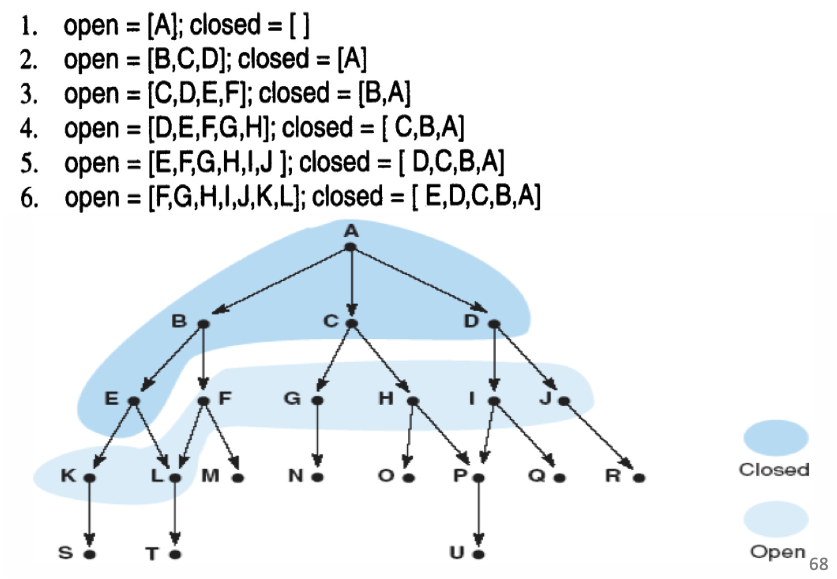
\includegraphics[scale=0.3]{images/breadth-first.png}

\bulletPoint{Famous Pdfs}:\quad

$\text{Bern}(x | \theta) = \theta^x (1 - \theta)^{1-x}=\theta^{\mathbbm{1}\{x=1\}} (1 - \theta)^{\mathbbm{1}\{x=0\}}$.
$\text{Unif}(x | a, b) = \frac{1}{b-a}  \mathbbm{1}\{a \leq x \leq b\}$.\quad
$\text{Exp}(x | \lambda) = \lambda e^{-\lambda x} \mathbbm{1}\{x \geq 0\}$.
$\text{Bin}(x | n, \theta) = \binom{n}{x} \theta^x (1 - \theta)^{n-x}$
where $\binom{n}{x} = \frac{n!}{x!(n-x)!}$.
$\text{Beta}(\theta | a, b) = \frac{\Gamma(a+b)}{\Gamma(a) \Gamma(b)} \theta^{a-1} (1-\theta)^{b-1}$.
$\Gamma(x) = \int_0^\infty t^{x-1} e^{-t} dt$ for $x \in \mathbb{R}$.

\bulletPoint{Probability Basics}:

\begin{itemize}[label=$\cdot$,leftmargin=0pt]
\item$\mathbb{P}((X,Y) \in A) = \int_A p(x,y) \,dx\,dy$. \quad
$p(x) = \int_{-\infty}^{\infty} p(x,y) \,dy$.\quad
$p(y | x) = \frac{p(x,y)}{p(x)}$.
\item$p(x,y) = p(x)p(y | x)$, 
If \(X\) and \(Y\) are independent, then \( p(x,y) = p(x)p(y) \).

\item\textbf{Likelihood of i.i.d. dataset:} 
$p(\mathcal{D}) = \prod_{i=1}^{n} p(x_i)$ or $\log p(\mathcal{D}) = \sum_{i=1}^{n} \log p(x_i)$. 
where dataset \( \mathcal{D} = \{x_1, \dots, x_n\} \) is i.i.d.
\item\textbf{Bayes' theorem:}
$p(x | y) = \frac{p(x,y)}{p(y)} = \frac{p(y | x) p(x)}{p(y)}$.
\item\textbf{Expectation:}  % Expectation
$\mathbb{E}[X] = \int_{-\infty}^{\infty} x p(x) \,dx, \quad \mathbb{E}[g(X)] = \int_{-\infty}^{\infty} g(x) p(x) \,dx$,\quad
$\mathbb{E}[X + Y] = \mathbb{E}[X] + \mathbb{E}[Y]$,\quad$\mathbb{E}[X \mid Y = y] = \int_{-\infty}^{\infty} x p(x \mid y) \,dx$,\quad
$\mathbb{E}[f(X) g(Y) \mid Y = y] = \mathbb{E}[f(X) \mid Y = y] g(y)$.
\item\textbf{Variance and Covariance:}  % Variance and Covariance
$\text{var}(X) = \mathbb{E}[(X - \mathbb{E}[X])^2] = \mathbb{E}[X^2] - \mathbb{E}[X]^2$,\quad
$\text{cov}(X,Y) = \mathbb{E}[(X - \mathbb{E}[X])(Y - \mathbb{E}[Y])] = \mathbb{E}[XY] - \mathbb{E}[X] \mathbb{E}[Y]$,\quad
$\text{var}(X + Y) = \text{var}(X) + \text{var}(Y) + 2 \text{cov}(X,Y)$.
\item \textbf{Vector Variables:}
$
\mathbf{x} =
\begin{bmatrix}
x_1 & x_2 & \cdots & x_n
\end{bmatrix}^{\top}, \quad
\mathbb{E}[\mathbf{x}] =
\begin{bmatrix}
\mathbb{E}[x_1] & \mathbb{E}[x_2] & \cdots & \mathbb{E}[x_n]
\end{bmatrix}^{\top}
$\quad
$\text{If } \mathbf{A} \text{ is a deterministic matrix, } \mathbb{E}[\mathbf{A} \mathbf{x}] = \mathbf{A} \mathbb{E}[\mathbf{x}].$\quad
$\text{Covariance: } \text{cov}(\mathbf{x}) = \mathbf{\Sigma}_{xx} = \mathbb{E}[(\mathbf{x} - \mathbb{E}\mathbf{x})(\mathbf{x} - \mathbb{E}\mathbf{x})^\top],$\quad
$\text{cov}(\mathbf{A} \mathbf{x}) = \mathbf{A} \, \text{cov}(\mathbf{x}) \mathbf{A}^\top$\quad
$\text{Cross-covariance: } \text{cov}(\mathbf{x}, \mathbf{y}) = \mathbf{\Sigma}_{xy} = \mathbb{E}[(\mathbf{x} - \mathbb{E}\mathbf{x})(\mathbf{y} - \mathbb{E}\mathbf{y})^\top]$
\item \textbf{Matrix Calculus:}
$\frac{\partial (\mathbf{a}^\top \mathbf{x})}{\partial \mathbf{x}} = \mathbf{a}, \quad
\frac{\partial (\mathbf{x}^\top \mathbf{A} \mathbf{x})}{\partial \mathbf{x}} = (\mathbf{A} + \mathbf{A}^\top) \mathbf{x}$\quad
$\frac{\partial (\mathbf{a}^\top \mathbf{X} \mathbf{b})}{\partial \mathbf{X}} = \mathbf{a} \mathbf{b}^\top$, \quad
$\frac{\partial \det(\mathbf{X})}{\partial \mathbf{X}} = \det(\mathbf{X}) (\mathbf{X}^{-1})^\top$, \quad
$\frac{\partial (\mathbf{a}^\top \mathbf{X}^{-1} \mathbf{b})}{\partial \mathbf{X}} = -(\mathbf{X}^{-1})^\top \mathbf{a} \mathbf{b}^\top (\mathbf{X}^{-1})^\top$

\end{itemize}
% \textbf{Parametric vs. Non-Parametric Models}
\bulletPoint{Parametric vs. Non-Parametric Models}

\begin{itemize}[leftmargin=0pt]
\item • A parametric model assumes a fixed number of parameters. It usually belongs to a predefined family of distributions: 
\( p(x,y) = p(x,y \mid \theta) \) or \( p(x) = p(x \mid \theta) \). \\
 1. Faster to train (find “optimal” \( \theta \)). 2. Stronger assumptions about the data distribution. 
\item • A non-parametric model the number of parameters grows with the amount of training data:
  1. More flexible.
  2. Can be computationally intractable for large datasets.
\end{itemize}

\bulletPoint{Bayesian Inference:} \quad

Given a parametric model, the posterior is derived as: $p(\theta \mid x) = \frac{p(x \mid \theta) p(\theta)}{p(x)} \propto p(x \mid \theta) p(\theta)$,
where $p(x)$ is a normalization constant.
If $p(x) \propto f(x)$ for some function $f(x)$, then $p(x) = c f(x)$ with 
$c = \left( \int f(x) dx \right)^{-1}$.

\bulletPoint{Conjugate Distributions:} \quad

If prior and posterior share the same form, they are conjugate:
$p(\theta \mid x) \propto p(x \mid \theta) p(\theta)$.
The prior $p(\theta)$ is called the conjugate prior of the likelihood $p(x \mid \theta)$.\\
1. Allows for analytical closed form solutions and easy to interpret. 
2. May lack flexibility to complex data, requiring MCMC.


\bulletPoint{Conjugate Prior for Binomial:} \quad

Given $s \sim \text{Bin}(n, \theta)$ and prior $\theta \sim \text{Beta}(a, b)$, the posterior is:
$p(\theta \mid s) \propto \text{Bin}(s \mid \theta, n) \cdot \text{Beta}(\theta \mid a, b)$
$\propto \theta^s (1 - \theta)^{n-s} \cdot \theta^{a-1} (1 - \theta)^{b-1}$
$\propto \theta^{s+a-1} (1 - \theta)^{n-s+b-1}$. 
Thus, the posterior follows:
$p(\theta \mid s) = \text{Beta}(\theta \mid s + a, n - s + b)$

\bulletPoint{Categorical Distribution:} \quad

• A categorical variable $X$ follows:
$\text{Cat} (x \mid \theta_1, \dots, \theta_K)$ with parameters $\theta_k \geq 0, \sum_{k=1}^{K} \theta_k = 1$;
$\text{Cat} (x \mid \theta_1, \dots, \theta_K)=\theta_x$.

• Given i.i.d. samples $X_i \sim \text{Cat}(\theta_1, \dots, \theta_K)$, the joint probability of $\mathcal{D} = \{X_1, \dots, X_n\}$ is: 
$p(\mathcal{D}) = \prod_{i=1}^{n} \text{Cat}(x_i \mid \theta_1, \dots, \theta_K) = \prod_{i=1}^{n} \prod_{k=1}^{K} \theta_k^{\mathbbm{1}\{x_i = k\}}$. 
Using count notation $N_k = \sum_{i=1}^{n} \mathbbm{1}\{x_i = k\}$, we get:
$p(\mathcal{D}) = \prod_{k=1}^{K} \theta_k^{N_k}$.


\bulletPoint{Gaussian (Normal) Distribution:} \quad

A random variable $X$ follows a normal distribution:
$\mathcal{N}(x \mid \mu, \sigma^2) = \frac{1}{\sqrt{2\pi\sigma^2}} e^{-\frac{1}{2\sigma^2} (x-\mu)^2}$.

If $X \sim \mathcal{N}(\mu, \sigma^2)$, then:
$aX \sim \mathcal{N}(a\mu, a^2\sigma^2)$ for any $a \in \mathbb{R}$
$X + c \sim \mathcal{N}(\mu + c, \sigma^2)$. 
If $Z \sim \mathcal{N}(0,1)$, then $X = \sigma Z + \mu \sim \mathcal{N}(\mu, \sigma^2)$. 
If $X \sim \mathcal{N}(\mu, \sigma^2)$ and $Y \sim \mathcal{N}(\xi, \nu^2)$ are independent:
$X + Y \sim \mathcal{N}(\mu + \xi, \sigma^2 + \nu^2)$.


\bulletPoint{Multivariate Gaussian Distribution:} \quad

A random vector $\mathbf{X}$ follows a multivariate normal distribution:
$\mathcal{N}(\mathbf{x} \mid \boldsymbol{\mu}, \boldsymbol{\Sigma}) = \frac{1}{(2\pi)^{K/2} (\det \boldsymbol{\Sigma})^{1/2}} \exp \left( -\frac{1}{2} (\mathbf{x} - \boldsymbol{\mu})^\top \boldsymbol{\Sigma}^{-1} (\mathbf{x} - \boldsymbol{\mu}) \right)$. 

• $\mathbf{X} = [X_1, \dots, X_n]^\top$ is \textit{jointly Gaussian} if for any vector $\mathbf{a} \in \mathbb{R}^n$, the linear combination: $\mathbf{a}^\top \mathbf{X} = \sum_{i=1}^{n} a_i X_i$ is Gaussian. 

• If $\mathbf{Z} \sim \mathcal{N}(\mathbf{0}, \mathbf{I})$, then: $\mathbf{X} = \mathbf{A} \mathbf{Z} + \boldsymbol{\mu}$  
is jointly Gaussian with mean and covariance: 
$\mathbb{E}[\mathbf{X}] = \boldsymbol{\mu}, \quad \text{cov}(\mathbf{X}) = \mathbf{A} \mathbf{A}^\top$. 

• $\boldsymbol{\mu} = 
\begin{bmatrix} \mu_X \\ \mu_Y \end{bmatrix}, \quad
\boldsymbol{\Sigma} = 
\begin{bmatrix} \sigma_X^2 & \text{cov}(X,Y) \\ \text{cov}(X,Y) & \sigma_Y^2 \end{bmatrix}$.\quad $\rho_{X,Y} = \frac{\text{cov}(X,Y)}{\sigma_X \sigma_Y}$.

\bulletPoint{Likelihood Functions for Common Distributions:}\quad

\textbf{1. Bernoulli:} If $x_i \sim \text{Bern}(\theta)$ i.i.d., where $\theta \in [0,1]$, then:
$p(\mathcal{D} \mid \theta) = \theta^{N_1} (1 - \theta)^{N_0}, \quad N_k = \sum_{i=1}^{n} \mathbbm{1}\{x_i = k\}$. 

\textbf{2. Exponential:} If $x_i \sim \text{Exp}(\lambda)$ i.i.d., where $\lambda > 0$, then:
$p(\mathcal{D} \mid \lambda) = \lambda^n \exp \left( -\lambda \sum_{i=1}^{n} x_i \right)$. 

\textbf{3. Gaussian:} If $x_i \sim \mathcal{N}(\mu, \sigma^2)$ i.i.d., then $\theta = (\mu, \sigma^2)$ and:
$p(\mathcal{D} \mid \theta) = \frac{1}{(2\pi)^{n/2} \sigma^n} \exp \left( -\frac{1}{2\sigma^2} \sum_{i=1}^{n} (x_i - \mu)^2 \right)$.


\bulletPoint{Maximum Likelihood Estimation (MLE):}\quad

The MLE of parameter $\theta$ is: $\theta_{\text{ML}} = \arg\max_{\theta} p(\mathcal{D} \mid \theta)$.
For i.i.d. data $\mathcal{D} = \{x_1, \dots, x_n\}$, we maximize the log-likelihood:
$\log p(\mathcal{D} \mid \theta) = \sum_{i=1}^{n} \log p(x_i \mid \theta)$. 

\textbf{Bernoulli MLE:} If $x_i \sim \text{Bern}(\theta)$, then: $p(\mathcal{D} \mid \theta) = \theta^{N_1} (1 - \theta)^{N_0}$,
$\log p(\mathcal{D} \mid \theta) = N_1 \log \theta + N_0 \log (1 - \theta)$. Solving $\frac{\partial}{\partial \theta} \log p(\mathcal{D} \mid \theta) = 0$:
$\theta_{\text{ML}} = \frac{N_1}{N_0 + N_1} = \frac{N_1}{n}$. 

\textbf{Exponential MLE:} If $x_i \sim \text{Exp}(\lambda)$, then: $\log p(\mathcal{D} \mid \lambda) = n \log \lambda - \lambda \sum_{i=1}^{n} x_i$.
Solving $\frac{\partial}{\partial \lambda} \log p(\mathcal{D} \mid \lambda) = 0$: $\lambda_{\text{ML}} = \frac{n}{\sum_{i=1}^{n} x_i}$.


\bulletPoint{Linear Regression Model:}\quad

$\mathbf{x} = (x_1, x_2, \dots, x_D)$, 
$y = \mathbf{w}^\top \mathbf{x} + \epsilon, $ $ \epsilon \sim \mathcal{N}(0, \sigma^2)$.\\
Thus, the likelihood is:
$p(y \mid \mathbf{x}, \mathbf{w}) = \mathcal{N}(y \mid \mathbf{w}^\top \mathbf{x}, \sigma^2)$. \\
\textbf{Basis Function Expansion:} model non-linear relationships using basis functions:
$
\phi(\mathbf{x}) =
\begin{bmatrix}
\varphi_1(\mathbf{x}) & \varphi_2(\mathbf{x}) & \cdots & \varphi_M(\mathbf{x})
\end{bmatrix}^{\top}
$
, \quad
$y = \mathbf{w}^\top \phi(\mathbf{x}) + \epsilon$; 
For $\mathbf{x} = \begin{bmatrix} x_1 \\ x_2 \end{bmatrix}$, $\phi(\mathbf{x}) = [1, x_1, x_2, x_1^2, x_2^2]$,
$y = w_1 + w_2 x_1 + w_3 x_2 + w_4 x_1^2 + w_5 x_2^2 + \epsilon$. \\
\textbf{MLE for $\mathbf{w}$:} Given i.i.d. training data $\mathcal{D} = \{(\mathbf{x}_i, y_i)\}$, 
$\log p(\mathbf{y} \mid \mathbf{\Phi}, \mathbf{w}) = -\frac{1}{2\sigma^2} \|\mathbf{\Phi} \mathbf{w} - \mathbf{y} \|^2 + \text{const}$,
where $\mathbf{\Phi} = [\mathbf{x}_1 \dots \mathbf{x}_n]^\top$ is the design matrix.
Maximizing w.r.t. $\mathbf{w}$ gives the least squares solution:
$\mathbf{w}_{\text{ML}} = (\mathbf{\Phi}^\top \mathbf{\Phi})^{-1} \mathbf{\Phi}^\top \mathbf{y}$. \\


\bulletPoint{Model Evaluation Metrics:}\quad

• $\text{RSS} = \sum_{i=1}^{n} (y_i - \hat{y}_i)^2$. \quad
• $\text{RMSE} = \sqrt{\frac{1}{n} \text{RSS}}$. \\
• $R^2 = 1 - \frac{\text{RSS}}{\text{TSS}} = 1 - \frac{\text{RSS}}{\sum_{i=1}^{n} (y_i - \bar{y})^2}$,

\bulletPoint{Maximum A Posteriori (MAP) Estimation:}\quad

• The MAP estimate maximizes the posterior:
$\theta_{\text{MAP}} = \arg\max_{\theta} p(\theta \mid \mathcal{D})$. Using Bayes' theorem: $p(\theta \mid \mathcal{D}) \propto p(\mathcal{D} \mid \theta) p(\theta)$,
$\log p(\theta \mid \mathcal{D}) = \log p(\mathcal{D} \mid \theta) + \log p(\theta) + \text{const}$. 

• Given:
$p(\mathcal{D} \mid \theta) = \theta^{N_1} (1 - \theta)^{N_0}, \quad p(\theta) = \text{Beta}(\theta \mid a, b)$,
$\log p(\mathcal{D} \mid \theta) p(\theta) = (N_1 + a - 1) \log \theta + (N_0 + b - 1) \log(1 - \theta)$.
Solving $\frac{\partial}{\partial \theta} \log p(\mathcal{D} \mid \theta) = 0$:
$\theta_{\text{MAP}} = \frac{N_1 + a - 1}{n + a + b - 2}$.

\bulletPoint{Classification and Naïve Bayes:}\quad

• Classification Rule: Given feature vector $\mathbf{x}$ and class label $y \in \{1, \dots, K\}$,
$\delta(\mathbf{x}) = k$ if $p(y = k \mid \mathbf{x})$ is maximized. \\
• Naïve Bayes Classifier: Assuming conditional independence,
$p(\mathbf{x} \mid y = c, \theta) = \prod_{d=1}^{D} p(x_d \mid \theta_{dc})$. Using Bayes' rule: $p(y = c \mid \mathbf{x}, \theta) \propto \pi(c) \prod_{d=1}^{D} p(x_d \mid \theta_{dc})$, where $\pi(c)$ is the prior probability of class $c$.


\bulletPoint{Mixture Models and Gaussian Mixture Model (GMM):}\quad

• Suppose an observation $\mathbf{x}$ can be generated from one of $K$ possible probability density functions (pdfs):
 $p(\mathbf{x} \mid \boldsymbol{\eta}_1), \dots, p(\mathbf{x} \mid \boldsymbol{\eta}_K)$.
The generating index $z$ follows a categorical distribution: $p(z) = \text{Cat}(z \mid \boldsymbol{\pi})$.
Since $z$ is unobserved, it is a \textbf{latent variable}. The marginal distribution is:
 $p(\mathbf{x} \mid \boldsymbol{\theta}) = \sum_{k=1}^{K} \pi(k) p(\mathbf{x} \mid \boldsymbol{\eta}_k)$,
 where $\boldsymbol{\theta} = (\boldsymbol{\pi}, \{ \boldsymbol{\eta}_k \}_{k=1}^{K})$. 

• GMM: $p(\mathbf{x} \mid \boldsymbol{\theta}) = \sum_{k=1}^{K} \pi(k) \mathcal{N} (\mathbf{x} \mid \boldsymbol{\mu}_k, \boldsymbol{\Sigma}_k)$,
 where $\boldsymbol{\theta} = (\boldsymbol{\pi}, \{ \boldsymbol{\mu}_k, \boldsymbol{\Sigma}_k \}_{k=1}^{K})$. 
Given i.i.d. observations $\mathbf{x}_1, \mathbf{x}_2, \dots, \mathbf{x}_n$, $p(\mathbf{x}_i \mid \boldsymbol{\theta}) = \sum_{k=1}^{K} \pi(k) p(\mathbf{x}_i \mid \boldsymbol{\eta}_k)$.\\
$\log p(\mathbf{x}_1, \dots, \mathbf{x}_n \mid \boldsymbol{\theta}) = \sum_{i=1}^{n} \log \sum_{k=1}^{K} \pi(k) p(\mathbf{x}_i \mid \boldsymbol{\eta}_k)$.

\bulletPoint{Algorithmic Issues in Mixture Models:}\quad

• Singularity:
If for some $k$, we set $\boldsymbol{\mu}_k = \mathbf{x}_i$ and $\sigma_k \to 0$, then:
$\mathcal{N}(\mathbf{x}_i \mid \boldsymbol{\mu}_k, \sigma_k \mathbf{I}) \propto \frac{1}{\sigma_k} \to \infty$. 

• Unidentifiability:
no unique global optimum for log-likelihood function. 

• Optimization Challenges: non-convex, hard to solve. 

• If latent variables $z_1, \dots, z_n$ are observed, the likelihood simplifies to:
$\log p((\mathbf{x}_1, z_1), \dots, (\mathbf{x}_n, z_n) \mid \boldsymbol{\theta}) = \sum_{i=1}^{n} \big( \log \pi[z_i] + \log p(\mathbf{x}_i \mid \boldsymbol{\eta}_{z_i}) \big)$.
much easier to maximize.


\bulletPoint{Gaussian Mixture Model (GMM):}\quad

• Observed data $\mathbf{x}_1, \dots, \mathbf{x}_n \in \mathbb{R}^{D}$ are generated from a mixture of $K$ Gaussian distributions:
$p(\mathbf{x} \mid \boldsymbol{\theta}) = \sum_{k=1}^{K} \pi(k) \mathcal{N} (\mathbf{x} \mid \boldsymbol{\mu}_k, \boldsymbol{\Sigma}_k)$
$\boldsymbol{\theta} = (\pi(k), \boldsymbol{\mu}_k, \boldsymbol{\Sigma}_k)_{k=1}^{K}$. 

• Complete data likelihood:
$\log p(\mathbf{y}_1, \dots, \mathbf{y}_n \mid \boldsymbol{\theta}) = \sum_{k=1}^{K} \sum_{i: z_i = k} \big( \log \pi(k) + \log \mathcal{N} (\mathbf{x}_i \mid \boldsymbol{\mu}_k, \boldsymbol{\Sigma}_k) \big).$. 

• The MLE estimates for $\boldsymbol{\mu}_k$ and $\boldsymbol{\Sigma}_k$:
$ \hat{\boldsymbol{\mu}}_k = \frac{1}{n} \sum_{i: z_i = k} \mathbf{x}_i, $ 
$ \hat{\boldsymbol{\Sigma}}_k = \frac{1}{n} \sum_{i: z_i = k} (\mathbf{x}_i - \hat{\boldsymbol{\mu}}_k)(\mathbf{x}_i - \hat{\boldsymbol{\mu}}_k)^{\top} $.

\bulletPoint{Expectation-Maximization (EM) Algorithm:}\quad

Complete data $\mathbf{y}$ can't be known directly. Still since $\log p(\mathbf{x} \mid \boldsymbol{\theta})$ is hard to optimize. Try maximize the expectation $\mathbb{E}_{p(\mathbf{y} \mid \mathbf{x}, \hat{\boldsymbol{\theta}})} \left[ \log p(\mathbf{y} \mid \boldsymbol{\theta}) \mid \mathbf{x}, \hat{\boldsymbol{\theta}} \right]$. 

\textbf{EM Steps:} 1. Initialize $\boldsymbol{\theta}^{(0)}$. \quad
2. \textbf{E-step}: Compute $Q(\boldsymbol{\theta} \mid \boldsymbol{\theta}^{(m)}) = \mathbb{E}_{p(\mathbf{y} \mid \mathbf{x}, \boldsymbol{\theta}^{(m)})} \left[ \log p(\mathbf{y} \mid \boldsymbol{\theta}) \mid \mathbf{x}, \boldsymbol{\theta}^{(m)} \right] = \int \log p(\mathbf{y} \mid \boldsymbol{\theta}) p(\mathbf{y} \mid \mathbf{x}, \boldsymbol{\theta}^{(m)}) d\mathbf{y}$. \quad

3. \textbf{M-step}: Update $\boldsymbol{\theta}$ by $\boldsymbol{\theta}^{(m+1)} = \arg\max_{\boldsymbol{\theta} \in \Theta} Q(\boldsymbol{\theta} \mid \boldsymbol{\theta}^{(m)})$. 

4. Repeat until convergence.

\bulletPoint{EM for GMM:}\quad

Given $\pi^{(0)}(k), \boldsymbol{\mu}_k^{(0)}, \boldsymbol{\Sigma}_k^{(0)}$ for $k=1,\dots,K$. 

$L^{(0)} = \frac{1}{n} \sum_{i=1}^{n} \log \left( \sum_{k=1}^{K} \pi^{(0)}(k) \mathcal{N} (\mathbf{x}_i \mid \boldsymbol{\mu}_k^{(0)}, \boldsymbol{\Sigma}_k^{(0)}) \right)$. 
\textbf{Repeat:}

1. \textbf{E-step:} Compute responsibilities:
    $r_{ik}^{(m)} = \frac{\pi^{(m)}(k) \mathcal{N} (\mathbf{x}_i \mid \boldsymbol{\mu}_k^{(m)}, \boldsymbol{\Sigma}_k^{(m)})}{\sum_{k'} \pi^{(m)}(k') \mathcal{N} (\mathbf{x}_i \mid \boldsymbol{\mu}_{k'}^{(m)}, \boldsymbol{\Sigma}_{k'}^{(m)})}$,  
    $n_k^{(m)} = \sum_{i=1}^{n} r_{ik}$. 
    
2. \textbf{M-step:} Update parameters:
    $\pi^{(m+1)}(k) = \frac{n_k^{(m)}}{n}$,  \quad
    $\boldsymbol{\mu}_k^{(m+1)} = \frac{1}{n_k^{(m)}} \sum_{i=1}^{n} r_{ik}^{(m)} \mathbf{x}_i$,  \quad
    $\boldsymbol{\Sigma}_k^{(m+1)} = \frac{1}{n_k^{(m)}} \sum_{i=1}^{n} r_{ik}^{(m)} (\mathbf{x}_i - \boldsymbol{\mu}_k^{(m+1)})(\mathbf{x}_i - \boldsymbol{\mu}_k^{(m+1)})^\top$. 

3. \textbf{Compute:}
    $L^{(m+1)} = \frac{1}{n} \sum_{i=1}^{n} \log \left( \sum_{k=1}^{K} \pi^{(m+1)}(k) \mathcal{N} (\mathbf{x}_i \mid \boldsymbol{\mu}_k^{(m+1)}, \boldsymbol{\Sigma}_k^{(m+1)}) \right)$. 

4. \textbf{untill:} $\lvert L^{(m+1)} - L^{(m)} \rvert \leq \epsilon$.
    

\bulletPoint{K-Means Algorithm}\quad

GMM with $\Sigma_k = \sigma^2 I$ and $\pi(k) = 1/K$ are fixed. Only $\mu_k$ are inferred. 

1. \textbf{E-step:} Assign each $x_i$ to its nearest cluster center: $k_i = \arg\min_{k} \|x_i - \mu_k^{(m)}\|^2$. Define hard assignment: $r_{ik}^{(m)} = 1$ if $k = k_i$, otherwise $r_{ik}^{(m)} = 0$. 

$Q(\theta \mid \theta^{(m)}) = -\frac{1}{2\sigma^2} \sum_{i=1}^{n} \|x_i - \mu_{k_i}^{(m)}\|^2 + \text{const}$. 

2. \textbf{M-step:} Update cluster centers: $\mu_k^{(m+1)} = \frac{1}{N_k} \sum_{i:k_i=k} x_i$, where $N_k = \sum_{i=1}^{n} \mathbbm{1}\{ k_i = k \}$. 

3. Update each cluster center using the mean of its assigned points.
    
\bulletPoint{EM Algorithm for MAP Estimation}\quad

Given data $\mathbf{x}$, the posterior is $p(\theta \mid \mathbf{x}) = \frac{p(\mathbf{x} \mid \theta) p(\theta)}{p(\mathbf{x})}$. The MAP estimate is $\theta_{MAP} = \arg\max_{\theta} \left( \log p(\mathbf{x} \mid \theta) + \log p(\theta) \right)$. 

\textbf{Algorithm:}

1. Pick initial guess $\theta^{(0)}$.

2. \textbf{E-step:} At iteration $m+1$, compute $Q(\theta \mid \theta^{(m)}) = \int p(\mathbf{y} \mid \mathbf{x}, \theta^{(m)}) \log p(\mathbf{y} \mid \theta) d\mathbf{y}$.

3. \textbf{M-step:} Update $\theta^{(m+1)} = \arg\max_{\theta} \left( Q(\theta \mid \theta^{(m)}) + \log p(\theta) \right)$.

4. Repeat until convergence. 

    
\bulletPoint{Markov Chains}\quad

A discrete-time sequence $\mathbf{x} = \{x[0], x[1], \dots\}$, where each $x[t] \in \{1, 2, \dots, M\}$, satisfies the Markov property:
$p(x[t] \mid x[1], \dots, x[t-1]) = p(x[t] \mid x[t-1])$

\bulletPoint{Transition Matrix}\quad

• Each row of $\mathbf{T}$ sums to one: $\sum_{j=1}^{M} T(i, j) = \sum_{j=1}^{M} p_{x[t] \mid x[t-1]}(j \mid i) = 1$.
$\mathbf{T}$ is a (row) stochastic matrix.

• Given initial distribution $\mathbf{p}_0 = [p_0(1), p_0(2), \dots, p_0(M)]$,  $\mathbf{p}_1 = \mathbf{p}_0 \mathbf{T}$. For general $t$, let $\mathbf{p}_t = [p_t(1), \dots, p_t(M)]$, then: $\mathbf{p}_t = \mathbf{p}_0 \mathbf{T}^t$.


\bulletPoint{MLE for Transition Matrix}\quad

• Estimate prior $\pi$ and transition matrix $\mathbf{T}$ from training data:
$p(x[0], \dots, x[t] \mid \pi, \mathbf{T}) = \pi(x[0]) \mathbf{T}(x[0], x[1])  \dots$ $\mathbf{T}(x[t-1], x[t])$.
Given $n$ observed sequences $\mathcal{D} = \{\mathbf{x}_1[0:t_1], \dots, \mathbf{x}_n[0:t_n]\}$, each of varying length $t_i+1$, assume all data points follow the same $\mathbf{T}$. 

• $\log p(\mathcal{D} \mid \pi, \mathbf{T}) = \sum_{i=1}^{n} \log \pi(x_i[0]) + \sum_{i=1}^{n} \sum_{t=1}^{t_i} \log \mathbf{T}(x_i[t-1], x_i[t])$
$= \sum_{x=1}^{M} N_x \log \pi(x) + \sum_{x=1}^{M} \sum_{y=1}^{M} N_{xy} \log \mathbf{T}(x, y)$. 

$N_x = \sum_{i=1}^{n} \mathbbm{1}(x_i[0] = x)$, $N_{xy} = \sum_{i=1}^{n} \sum_{t=1}^{t_i} \mathbbm{1}(x_i[t-1] = x, x_i[t] = y)$. 

• $\hat{\pi}(x) = \frac{N_x}{n}$, $\hat{\mathbf{T}}(x, y) = \frac{N_{xy}}{\sum_{z=1}^{M} N_{xz}}$. 
  
• May predict certain strings are impossible if data have zero count of certain states (this is a form of overfitting).

\bulletPoint{HMM: Hidden Markov Model}\quad

A hidden Markov model consists of:

• A discrete state Markov chain with \textbf{hidden states} or latent variables $z[t] \in \{1, \dots, M\}$, $t = 0,1,\dots$, with initial pdf $\pi$ and transition matrix $\mathbf{T}$.

• An observation model with emission probabilities $p(\mathbf{x}[t] \mid z[t]) = p(\mathbf{x}[t] \mid \phi_{z[t]})$, where $\phi = (\phi_1, \dots, \phi_M)$. 
Applications: 
(1) Long-range dependencies; 
(2) Speech recognition;
(3) Gene finding;
(4) Emission probabilities (Gaussian example). 

\bulletPoint{Baum-Welch Algorithm for HMM Training}\quad

1. Initialize $\theta^{(0)}$.

2. \textbf{E step}: Use Forward-Backward Algorithm to compute
    $\gamma_{i,t}(z) = p(z_i[t] = z | \mathbf{x}_i[0:t_i], \theta^{(m)}) \propto \alpha_j(z) \beta_j(z)$, 
    $\xi_{i,t}(z,z') = p(z_i[t-1] = z, z_i[t] = z' | \mathbf{x}_i[0:t_i], \theta^{(m)})$, 
    $\quad \propto \alpha_{t-1}(z) p(\mathbf{x}_i[t] | z_i[t]=z') \beta_t(z') p(z_i[t] = z' | z_i[t-1] = z)$. 

3. \textbf{M step}: Update parameters
    $\hat{\pi}(z) = \frac{\sum_{i=1}^{n} \gamma_{i,0}(z)}{n}$, 
    $\hat{T}(z,z') = \frac{\sum_{i=1}^{n} \sum_{t=1}^{t_i} \xi_{i,t}(z,z')}{\sum_u \sum_{i=1}^{n} \sum_{t=1}^{t_i} \xi_{i,t}(z,u)}$, 
    $\hat{\phi}_z$ = emission probability parameters.

4. Repeat E and M steps.
  
\bulletPoint{Inference in HMMs}\quad

• Filtering: Estimate latent state $p(z[t] | \mathbf{x}[0:t])$ using observations up to time $t$ ({Forward Algorithm}). 

• Smoothing: Estimate $p(z[t] | \mathbf{x}[0:T])$, using both past and future observations ({Forward-Backward Algorithm}). 

• Fixed-lag smoothing: Estimate $p(z[t-l] | \mathbf{x}[0:t])$ for online inference ({Forward-Backward Algorithm}). 

• Prediction: Estimate $p(z[t+h] | \mathbf{x}[0:t])$, where $h > 0$ is the prediction horizon:
$p(z[t+h] | \mathbf{x}[0:t]) = \sum_{z[t],...,z[t+h-1]} p(z[t+h] | z[t+h-1]) p(z[t+h-1] | z[t+h-2]) \cdots p(z[t+1] | z[t]) \cdot p(z[t] | \mathbf{x}[0:t])$. 

• MAP sequence: using Viterbi Algorithm, most probable sequence $\mathbf{z}^*[0:T] = \arg\max_{z[0:T]} p(z[0:T] | \mathbf{x}[0:T])$.


\bulletPoint{Sampling Using Cdf}\quad

If \( X \sim F \), then:
$\mathbb{P}(X \leq x) = F(x)$, \quad
Let \( U \sim \text{Unif}(0,1) \), define:
$X = F^{-1}(U)
\Rightarrow X \sim F$. 

$\mathbb{P}(F^{-1}(U) \leq x) = \mathbb{P}(U \leq F(x)) = F(x)$. 

\bulletPoint{Transformations}\quad

If \( Y = f(X) \), then \( p_Y(y) = \sum_{k=1}^K \frac{p_X(x_k)}{|f'(x_k)|} \), where \( x_k \) are the solutions to \( f(x) = y \)
\quad\textbf{Note:} Requires solving \( f(x) = y \) and knowing \( f'(x) \)


\bulletPoint{Rejection Sampling}\quad

• \( p(z) = \frac{1}{M} \tilde{p}(z) \), where \( M \) unknown. 
Choose proposal \( q(z) \), and constant \( k \geq \frac{\tilde{p}(z)}{q(z)} \) for all \( z \). 

• \( \text{supp}(p) \subseteq \text{supp}(q) \), where $\operatorname{supp} p = \overline{ \{ z : p(z) > 0 \} }$. 

• \textbf{Sampling Procedure:}
1. Sample \( z \sim q(z) \) \quad
2. Sample \( u \sim \text{Unif}[0, kq(z)] \) \quad
3. Accept \( z \) if \( u \leq \tilde{p}(z) \). 

• $\mathbb{P}(z\text{ accepted}) = \int \frac{\tilde{p}(z)}{kq(z)} q(z)\,dz = \frac{M}{k}$. \quad

• Choose smallest possible \( k \) s.t. \( kq(z) \geq \tilde{p}(z) \ \forall z \). \quad

• Accepted \( z \sim p(z) \)
$\mathbb{P}(z \leq z_0 \mid \text{accepted}) = \frac{1}{M} \int_{z \leq z_0} \tilde{p}(z)\,dz$
→ Accepted samples follow the CDF of \( p(z) \)

\bulletPoint{Importance Sampling}\quad

• Estimate expectation $\mathbb{E}_p[f(z)] = \int f(z)p(z)\,dz$, where $p(z)$ is hard to sample.  

• Use proposal $q(z)$ and importance weights $w(z) = \frac{p(z)}{q(z)}$, rewrite as  
$\mathbb{E}_p[f(z)] = \int f(z)w(z)q(z)\,dz \approx \frac{1}{n} \sum_{i=1}^n w(z_i)f(z_i)$, where $z_i \sim q(z)$. 

• $\text{supp}(f(\cdot)p(\cdot)) \subseteq \text{supp}(q)$. Keep all samples, no need $q(z) \geq p(z)$. Better matches well, if $q(z)$ is large where $|f(z)|p(z)$ is large. 

• If only know how to compute $p(z)$ and $q(z)$ up to normalizing constants, use normalized weights:   

$\mathbb{E}_p[f(z)] \approx \sum_{i=1}^n w_n(z_i)f(z_i)$, $w_n(z_i) = \frac{w(z_i)}{\sum_j w(z_j)}$.

\bulletPoint{Sampling Importance Resampling (SIR)}\quad

• Convert importance weighted samples into unweighted samples from $p(z)$. 

• \textbf{Steps:}

1. Sample $z_1,\dots,z_n$ from $q(z)$. 

2. Compute weights $w_n(z_1),\dots,w_n(z_n)$.

3. Resample with replacement from $\{z_1,\dots,z_n\}$ using weights $(w_n(z_1),\dots,w_n(z_n))$. 

• Each sample $\tilde{z}_i$ drawn from multinomial over $\{z_1,\dots,z_n\}$ with weights $w_n(z_i)$. 
asymptotically for large $n\to\infty$, 
$\mathbb{P}(\tilde{z} \leq a) = \sum_{i=1}^n w_n(z_i)\mathbbm{1}_{\{z_i \leq a\}} \to \int_{z \leq a} p(z)\,dz$. 

\bulletPoint{SIR for Bayesian Inference}\quad

• Take unnormalized $\tilde{p}(\theta) = p(\mathcal{D} \mid \theta)p(\theta)$, sample $\theta_1,\dots,\theta_n$ from $q(\theta) = p(\theta)$. 

• $w_n(\theta_i) = \frac{\tilde{p}(\theta_i)/q(\theta_i)}{\sum_j \tilde{p}(\theta_j)/q(\theta_j)} = \frac{p(\mathcal{D} \mid \theta_i)}{\sum_j p(\mathcal{D} \mid \theta_j)}$. 

• Resampling $\theta_1,\dots,\theta_n$ according to weights $(w_n(\theta_1),\dots,w_n(\theta_n))$. 

\bulletPoint{Sampling for EM}\quad

• Observed incomplete data $\mathbf{x}$, while complete is $\mathbf{(x,z)}$. 
Need to compute:
$Q(\theta \mid \theta^{(m)}) = \int p(\mathbf{z} \mid \mathbf{x}, \theta^{(m)}) \log p(\mathbf{x}, \mathbf{z} \mid \theta)\,dz$. 

• $Q(\theta \mid \theta^{(m)}) \approx \frac{1}{n} \sum_{i=1}^n \log p(\mathbf{x}, \mathbf{z}_i \mid \theta)$, where $\mathbf{z}_i \sim p(\mathbf{z} \mid \mathbf{x}, \theta^{(m)})$. 

• Rejection and importance sampling not suitable for high-dimensional $\mathbf{z}$ → need MCMC methods

\bulletPoint{Stationary Distribution}\quad

Consider homogeneous Markov chain with transition probability $p(x_t = y \mid x_{t-1} = x) = \mathbf{T}(x, y)$. 
$\pi$ is a stationary distribution if $\sum_x \pi(x)\mathbf{T}(x, y) = \pi(y)$ for all states $y$. 
Also called invariant distribution — does not change over time in the chain. 
If $M$ states, $\mathbf{T}$ is an $M \times M$ matrix with $\pi \mathbf{T} = \pi$. 

\bulletPoint{Asymptotic Steady State}\quad

Initial distribution: $\pi_0$. 
Markov evolution: $\pi_1 = \pi_0 \mathbf{T}, \ \pi_2 = \pi_1 \mathbf{T}, \ \dots, \ \pi_k = \pi_0 \mathbf{T}^k$. 
If the limit $\pi = \lim_{k \to \infty} \pi_k = \lim_{k \to \infty} \pi_0 \mathbf{T}^k$ exist,$\pi$ must satisfy $\pi \mathbf{T} = \pi$ → a stationary distribution


\bulletPoint{Reversible Markov Chain (MC)}\quad

• Sufficient condition but not necessary condition for $\pi$ to be stationary: $\pi(x)\mathbf{T}(x,y) = \pi(y)\mathbf{T}(y,x)$ for all $x, y$  
→ This chain is \textit{reversible}. 
Summing both sides over $x$:  
$\sum_x \pi(x)\mathbf{T}(x,y) = \sum_x \pi(y)\mathbf{T}(y,x) = \pi(y)\sum_x \mathbf{T}(y,x) = \pi(y)$. 

• Sampling from a distribution $\pi(x)$: 
Design transition $\mathbf{T}(x,y)$ such that 
(1) All the ergodicity conditions hold  
(2) Usually make $\mathbf{T}$ reversible and aperiodic  
(3) $\pi(x)$ is stationary distribution. 

• MCMC basis:
Generate sample path for the Markov chain $z_0, z_1, \dots, z_n$ starting from any $z_0$.   
If $n$ large, then $p(z_n) \approx \pi(z_n)$  
→ obtain samples from $\pi$


\bulletPoint{Metropolis-Hastings Algorithm} \quad

• Sample from $\pi(\mathbf{x})$ (e.g., $\mathcal{X} = \mathbb{R}^{1000}$). 
Assume we can compute unnormalized density $\tilde{\pi}(\mathbf{x})$. 
Choose transition probability $q(\mathbf{x}, \mathbf{y})$ that is irreducible, aperiodic, and easy to sample — this is the \textit{proposal distribution}. 

• Let $Z_0, Z_1, \dots$ be the chain states. At step $m$:

1. Let $\mathbf{x} = Z_{m-1}$.  

2. Sample $\mathbf{y} \sim q(\mathbf{x}, \cdot)$.   

3. Accept $\mathbf{y}$ with probability  
$A(\mathbf{x}, \mathbf{y}) = \min\left(1, \frac{\tilde{\pi}(\mathbf{y})q(\mathbf{y}, \mathbf{x})}{\tilde{\pi}(\mathbf{x})q(\mathbf{x}, \mathbf{y})} \right)$.   

4. If accepted, $Z_m = \mathbf{y}$; else $Z_m = Z_{m-1}$. 

• (1) Sequence $Z_0, Z_1, \dots$ is a Markov chain (only depends on $Z_{m-1}$)  
(2) Like rejection/importance sampling, does not need normalization constant of $\tilde{\pi}$  
(3) Suitable for high-dimensional $\pi(\mathbf{x})$ since sampling is from simple $q(\mathbf{x}, \cdot)$


\bulletPoint{Proposal Distributions}\quad

• MH chain $Z_0, Z_1, \dots$ is designed to converge to stationary distribution $\pi(\cdot)$.   
For large $m$, $Z_m \sim \pi$ approximately.   

• Burn-in period: discard first 1000 to 5000 samples

• Choice of Proposal Distribution:

1. $q(\mathbf{x}, \mathbf{y}) = q(\mathbf{y} - \mathbf{x})$ — \textit{random walk MH}.   

(1) $\mathbf{y} - \mathbf{x} \sim \mathcal{N}(0, \Sigma)$ — Gaussian centered at $\mathbf{x}$. \quad  

(2) $\mathbf{y} - \mathbf{x} \sim \text{Unif}[-\delta, \delta]^d$ — Uniform around $\mathbf{x}$.   \quad

(3) If $q(\mathbf{x}, \mathbf{y}) = q(\mathbf{y}, \mathbf{x})$, then  
$A(\mathbf{x}, \mathbf{y}) = \min\left(1, \frac{\tilde{\pi}(\mathbf{y})}{\tilde{\pi}(\mathbf{x})}\right)$  known as the Metropolis Algorithm. 

(4) Variance affects — small $\Rightarrow$ slow,\quad high $\Rightarrow$ high rejection rates.

2. Independence Chain MH: 
$q(\mathbf{x}, \mathbf{y}) = q(\mathbf{y})$, i.e. next state is independent of current. \quad  
Works well if $q(\mathbf{y})$ closely approximates $\pi(\mathbf{y})$ and is heavy-tailed

3. Exploiting Structure of $\pi$: 
Suppose $\pi(\mathbf{x}) \propto \psi(\mathbf{x}) h(\mathbf{x})$, with $h(\mathbf{x})$ is a density
that can be sampled from, bounded function $\psi(\mathbf{x})$. \quad  
Choose $q(\mathbf{x}, \mathbf{y}) = h(\mathbf{y})$, then:
$A(\mathbf{x}, \mathbf{y}) = \min\left(1, \frac{\tilde{\pi}(\mathbf{y})q(\mathbf{y}, \mathbf{x})}{\tilde{\pi}(\mathbf{x})q(\mathbf{x}, \mathbf{y})} \right)
= \min\left(1, \frac{\psi(\mathbf{y})h(\mathbf{y})h(\mathbf{x})}{\psi(\mathbf{x})h(\mathbf{x})h(\mathbf{y})} \right)
= \min\left(1, \frac{\psi(\mathbf{y})}{\psi(\mathbf{x})} \right)$


\bulletPoint{Proposal Variance} \quad

• Important to tune proposal variance $\sigma$. \quad

• $\sigma$ too small → slow convergence, high acceptance rate, takes a long time to explore the whole space. 

• $\sigma$ too large → big steps, low acceptance rate, stuck for long time. 

• Rules of thumb:
(1) Random walk MH: target acceptance rate of 0.25 to 0.5. 
(2) Independence chain MH: acceptance rate close to 1

\bulletPoint{Burn-In} \quad

Discard early samples before chain reaches stationary distribution. 
Hard to know when. E.g. $x_0 \sim \text{Unif}(\{0,1,\dots,20\})$, takes over 400 steps to "forget" initial state.

\bulletPoint{Thinning}\quad

Break dependencies between samples by taking every $d$-th sample. 
Useful when $\sigma$ is too large → MC stuck for long time at same location. 
Subsample every $d$ samples: $z_0, z_d, z_{2d}, \dots$

\bulletPoint{Gibbs Sampling}\quad

Special case of Metropolis-Hastings, for multivariate $p(z_1, \dots, z_d)$ (hard to sample jointly when $d$ is large). 
For each $i$, define $\mathbf{z}_{-i} = \{z_1,\dots,z_{i-1},z_{i+1},\dots,z_d\}$. 
If we can compute full conditionals $p(z_i \mid \mathbf{z}_{-i})$, we can perform Gibbs sampling:

• Initialize $(z_1^{(0)}, \dots, z_d^{(0)})$.   

• For each iteration $k$, sequentially sample:
$z_1^{(k)} \sim p(\cdot \mid z_2^{(k-1)}, \dots, z_d^{(k-1)})$  
$z_2^{(k)} \sim p(\cdot \mid z_1^{(k)}, z_3^{(k-1)}, \dots)$  
...  
$z_j^{(k)} \sim p(\cdot \mid z_1^{(k)}, \dots, z_{j-1}^{(k)}, z_{j+1}^{(k-1)}, \dots)$  
...
$z_d^{(k)} \sim p(\cdot \mid z_1^{(k)}, \dots, z_{d-1}^{(k)})$. 

• Discard burn-in samples.

• Generating Approximate i.i.d. Samples: 
(1) Run $r$ independent Gibbs chains of length $m$, use final sample from each sequence.
(2) Run one long sequence, discard burn-in, take every $d$-th sample. 

• Getting conditionals distributions:
$p(z_1 \mid z_2, \dots, z_d) = \frac{p(z_1, \dots, z_d)}{p(z_2, \dots, z_d)}$
(1) Start with joint $p(z_1, \dots, z_d)$.   
(2) Drop constants not depend on $z_1$.   
(3) Use knowledge of well-known distributions to find the distribution $p(z_1 \mid z_2, \dots, z_d)$. 



%%%%%%%%%%%%%%%%%%%%%%%%%%%%%%%%%%%%%%%%%%%%%%%%%%%%%%%%%%%%%%%%%%%%%%%%%%%%%%%%%%%%%below is wlb's part


\bulletPoint{Introduction to NN and DL} \quad

• An artificial neuron computes $y = f\left(\sum_{j=0}^{m} w_j x_j\right)$ with $x_0 = 1$, $w_0 = b$. \quad
Common activations: sigmoid $f(x) = \frac{1}{1 + e^{-x}}$, ReLU $f(x) = \max(0, x)$. 

• Binary output: $1$ if $\mathbf{w}^T \mathbf{p} + b > 0$, else $0$. \quad
Decision boundary: $\mathbf{w}^T \mathbf{p} + b = 0$. \quad +1 from negative to positive.

• OR Gate Perceptron Design:
Given $\mathbf{w} = [1, 1]^T$, point $\mathbf{p} = [0, 0.5]^T$ lies on the boundary. \quad
Then $1 \cdot 0 + 1 \cdot 0.5 + b = 0 \Rightarrow b = -0.5$. 

• AND Gate Perceptron Design:
Given $\mathbf{w} = [1, 1]^T$, point $\mathbf{p} = [0, 1.5]^T$ lies on the boundary. \quad
Then $1 \cdot 0 + 1 \cdot 1.5 + b = 0 \Rightarrow b = -1.5$. 

• XOR and Multi-Layer Perceptron:
Single-layer fails on XOR. Use hidden layer: \quad
Neuron 1: $\mathbf{w}_1 = [1,1]^T$, $b = -0.5$; Neuron 2: $\mathbf{w}_2 = [-1,-1]^T$, $b = 1.5$. \quad
Output neuron AND: $\mathbf{w}_{\text{out}} = [1,1]$, $b = -1.5$. 

• Forward Propagation: 
Given $W_1, W_2, W_3$, $b_1, b_2, b_3$, input $\mathbf{p}$, compute: \quad
$\mathbf{h}_1 = \sigma(W_1 \mathbf{p} + b_1)$, $\mathbf{h}_2 = \sigma(W_2 \mathbf{h}_1 + b_2)$, $\hat{y} = \sigma(W_3 \mathbf{h}_2 + b_3)$.

• Universal Approximation Theorem:
(1) Approximating Arbitrary Decision Regions with 3-Layer MLP; Approximating a Function with 2-Layer MLP.
(2) A hidden layer of nonconstant, bounded, and continuous neurons (with weights
and biases), plus a linear output neuron (with weights but without bias) can
approximate any continuous function to any arbitrary accuracy if there are
enough hidden neurons. 

\bulletPoint{Feedforward Computation} \quad

A multilayer NN maps input $x$ to output $y$ via: 
$y = f(x) = \sigma(W_L \sigma(W_{L-1} \dots \sigma(W_1 x + b_1) \dots + b_{L-1}) + b_L)$. \quad

All layers use weight matrices $W_i$ and bias vectors $b_i$. 

\bulletPoint{NN terminology Basics} \quad

• Classification: last layer = softmax, loss = cross-entropy. \quad

• Regression: last layer = linear, loss = MSE. \quad

• "2-layer NN(1-hidden-layer NN)" = input + 1 hidden + output. \quad

• "3-layer NN(2-hidden-layer NN)" = input + 2 hidden + output.

\bulletPoint{Activation Functions} \quad

• Sigmoid: $\sigma(x) = \frac{1}{1 + e^{-x}}$, output in $[0,1]$, saturates. \quad

• Tanh: $\tanh(x)=2\sigma(2x)-1$, output in $[-1,1]$, zero-centered. \quad

• ReLU: $\max(0, x)$, avoids vanishing gradient, fast to compute. \quad

• Leaky ReLU: $f(x) = \alpha x$ if $x < 0$, else $x$, avoids dead neurons. \quad

• Linear: $f(x) = cx$, used in regression output layer. 
Also known as identity activation function.

• Softmax: $\text{softmax}(z_i) = \frac{e^{z_i}}{\sum_j e^{z_j}}$, output is probability distribution.\quad
• Maxout.\quad • Exponential Linear Unit (ELU). 

\bulletPoint{Data Preprocessing} \quad

• Standardization: zero mean, unit variance. \quad
$x' = \frac{x - \mu}{\sigma}$ \quad

• Normalization: scale to $[0, 1]$ or $[-1, 1]$: $x' = \frac{x - \min(x)}{\max(x) - \min(x)}$

\bulletPoint{Loss Functions} \quad

• Classification: Cross-entropy loss: 
$\mathcal{L}(\theta) = -\sum_{k=1}^K y_k \log \hat{y}_k$. 

• Regression: 

Mean squared error (MSE): $\mathcal{L}(\theta) = \frac{1}{n} \sum_i (y_i - \hat{y}_i)^2$. 

Mean absolute error (MAE): $\frac{1}{n} \sum_i |y_i - \hat{y}_i|$

\bulletPoint{Gradient Descent (GD)} \quad

1. \textbf{Initialization:} Randomly initialize the model parameters $\theta^0$. Set $\theta^{\text{old}} = \theta^0$.

2. Compute the gradient of the loss function at $\theta^{\text{old}}$: $\nabla \mathcal{L}(\theta^{\text{old}})$.

3. Update the parameters:
$\theta^{\text{new}} = \theta^{\text{old}} - \alpha \nabla \mathcal{L}(\theta^{\text{old}})$
where $\alpha$ is the learning rate.

4. Set $\theta^{\text{old}} = \theta^{\text{new}}$ and return to step 2 (repeat until terminating).

GD does not guarantee reaching a global minimum.

• Backpropagation: Combines forward pass + backward pass using chain rule to compute gradients of loss w.r.t. weights. 

• Batch GD: compute gradients over full dataset. 

• Mini-batch GD: over subset (e.g., 32 to 256 samples). Mini-batch gradient approximates the full training set gradient well.

• SGD: mini-batch size = 1, fast but noisy. Less used. 

\bulletPoint{GD with Momentum:}

• Momentum: $v_t = \beta v_{t-1} + (1-\beta) \nabla \mathcal{L}$, improves convergence. \quad

• Nesterov Momentum: lookahead at next step before computing gradient. (Skip)

• Adam: computes a weighted average of past gradients and weighted average of past squared gradients. 
• Other: RMSprop, Adagrad, Adadelta, Nadam, etc. 
• Most used: Adam, SGD with momentum.

\bulletPoint{Learning Rate (LR)} 

• Too small → slow convergence; Too large → divergence or oscillations. 
• LR scheduling: reduce $\alpha$ over time. 
Approaches: step decay, exponential/cosine decay, reduce by constant, warmup(increase then cool down).

\bulletPoint{Underfitting and Overfitting} 

• Underfitting: high train + validation error (too simple). 

• Overfitting: low train error, high validation error (too complex). 

\bulletPoint{Regularization Techniques} \quad

• $\ell_2$ regularization: $\mathcal{L}_{\text{reg}} = \mathcal{L}(\theta) + \lambda \sum_k \theta_k^2$, penalty for large.

• $\ell_1$ regularization: $\sum_k |\theta_k|$, perform worse than $\ell_2$. \quad

• Elastic net: mix of $\ell_1$ and $\ell_2$. \quad
• Dropout: randomly deactivate neurons during training (e.g., $p=0.5$). \quad
• Early stopping: monitor validation loss, stop if no improvement after $n$ epochs.

\bulletPoint{Batch Normalization} \quad

• Normalize each mini-batch: $\hat{x} = \frac{x - \mu}{\sigma}$ \quad

• Less dependent on initialization. Normalizes activations. Reduces vanishing/exploding gradients. Reduces internal covariate shift.
Stabilizes training, enables higher learning rates. Common in CNNs.

\bulletPoint{Hyperparameter Tuning} \quad

• layer size, lr(schedule), optimizer, regularization, batch size, activation, loss f. \quad

• Methods: grid search(check all with step), random search, Bayesian optimization. Use k-fold cross-validation if data is limited.

\bulletPoint{Why MLP Fails on Images} \quad
MLPs are not translation invariant: shifting the input changes the output drastically. CNNs solve this with local receptive fields and shared weights.

\bulletPoint{Convolution Operation} \quad
• 1D: Convolution flips and slides a kernel $w$ over input $x$,

$(x * w)[n] = \sum_{k=-\infty}^{\infty} x[k] w[n-k]$

$x = [1, 2, 3, 4]$, $w = [5, 6, 7]$→$z = [5, 16, 34, 52, 45, 28]$

• 2D: Apply 2D filter over 2D image by elementwise multiplication and sum. Edge detectors highlight directional features.

\bulletPoint{Convolutional Neural Networks(CNNs)} \quad
• Parameter sharing via convolution filters. \quad
• Sparse connections via local receptive fields. \quad
• Translation invariance. \quad
• Fewer parameters than MLPs → faster training.

% CNNs use a convolutional operator for extracting data features. 

% • Allows parameter sharing, Efficient to train. 

% • Require fewer parameters than fully connected neural networks. 

% • CNNs are robust to spatial translations of objects in images. 

% • A convolutional filter slides across the image. 

\bulletPoint{Residual Networks (ResNets)} \quad
• Use identity skip connections: output = layer(x) + x. \quad
• Help prevent vanishing gradients. \quad

• Enable very deep models (e.g., 18, 50, 152 layers).

\bulletPoint{CNN Details} \quad
• Each filter spans full input depth. \quad
• Produces one activation map per filter. \quad
• Multiple filters produce stacked output (e.g., 6 filters → output depth = 6). 

\bulletPoint{CNN Architecture} \quad
Typical: [(CONV - ReLU)$\times N$ - POOL]$\times M$ - [FC - ReLU]$\times K$ - Softmax. \quad
Modern trends: deep models (VGG, ResNet), small filters ($3\times3$), less pooling.


\bulletPoint{Spatial Dimensions} \quad
For input of size $W_1 \times H_1 \times C$, filter size $F$, stride $S$, padding $P$, number of filters $K$:

it will produce an output of $W_2 \times H_2 \times K$
$W_2 = \frac{W_1 - F + 2P}{S} + 1$. Same for $H_2$. 

Number of parameters per filter: $F^2 C + 1$ (bias), \quad total: $K(F^2C + 1)$ for $K$ filters.\quad

\textbf{Example Calculation:} 
Input: $32 \times 32 \times 3$, Filters: $10$ of size $5 \times 5$, stride $1$, padding $2$ \quad
Output spatial size: $(32+2*2-5)/1 + 1 = 32$ → $32 \times 32 \times 10$ \quad
Params: $5*5*3 + 1 = 76$ per filter → total $760$ parameters.

\bulletPoint{Padding Strategy} \quad
Zero-padding preserves spatial size. To preserve size: use padding $P = \frac{F - 1}{2}$ if $S = 1$

\bulletPoint{Pooling Layer} \quad
• Reduces spatial size, parameters, overfitting. \quad

• Max pooling: keep largest value in window. \quad
• Avg pooling: keep mean value. \quad
• Output size: $W_2 = \frac{W_1 - F}{S} + 1$, same for $H_2$. \quad 

• 0 learnable parameters.

\bulletPoint{Flatten and FC Layer} \quad
• Flatten: convert activation map to 1D before FC. \quad
• FC: standard dense layer connects to all inputs.

\bulletPoint{Blank area for Appendix Notes}



\end{multicols*}

\end{document}